1. \begin{figure}[ht!]
\center{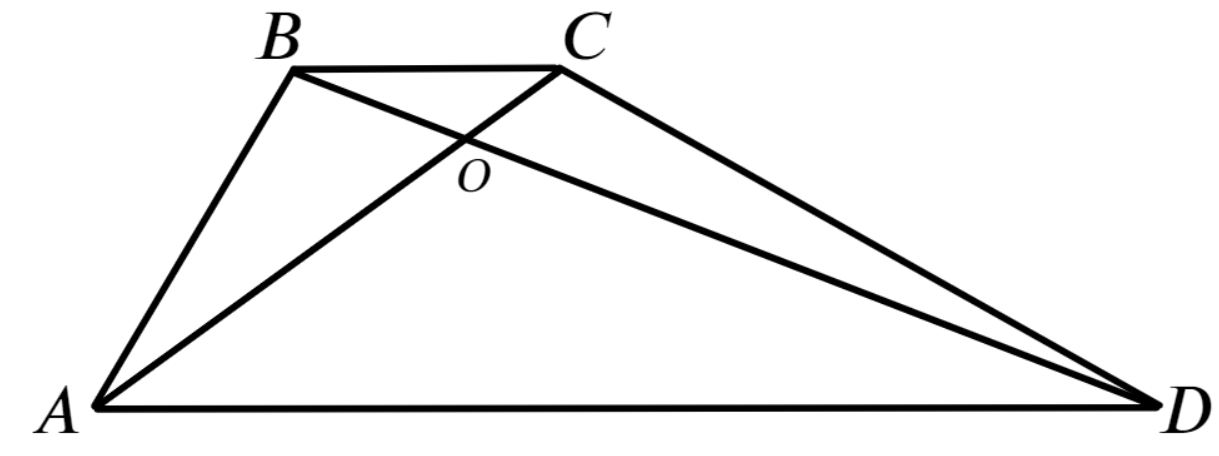
\includegraphics[scale=0.35]{g8-105.png}}
\end{figure}\\
Треугольники $AOD$ и $BOC$ подобны по двум углам ($\angle AOD$ и $\angle BOC$ вертикальные, $\angle BCO$ и $\angle OAD$ накрест лежащие). Раз
$\cfrac{S_{\Delta AOD}}{S_{\Delta BOC}}=16,$ коэффициент подобия равен $\sqrt{16}=4,$ поэтому $\cfrac{BC}{AD}=\cfrac{1}{4}.$\\
